\section{Análisis estático automatizado de código}

	\subsection{Error nº1: Memory leak}

		\subsubsection{Origen/explicación del error detectado}
		
			\paragraph{}En las siguientes dos capturas de pantalla se muestra el código fuente de las funciones \textit{modifica} y \textit{elimina\_dato} de la clase plantilla \textit{lista\_sin} de nuestra aplicación.
			
			\begin{figure}[H]
				\centering
				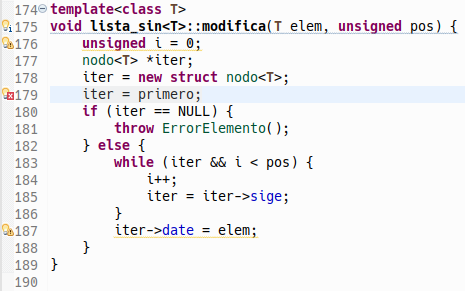
\includegraphics[scale=0.7]{img/captura42.png}
				\caption{Captura de pantalla de la función modifica}
				\label{captura42}
			\end{figure}
		
			\begin{figure}[H]
				\centering
				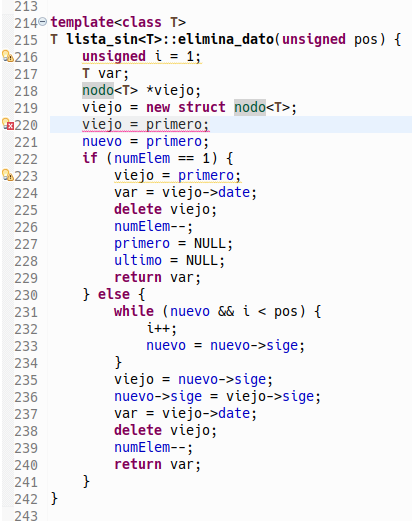
\includegraphics[scale=0.7]{img/captura45.png}
				\caption{Captura de pantalla de la función elimina\_dato}
				\label{captura45}
			\end{figure}
		
			\paragraph{}En la línea 179 cppchek nos indica que ha detectado un error de código, en concreto, se trata de un error de perdida de memoria para la variable \textit{iter}. Esto es debido a que en la línea 177 se declara la variable (la cual es un puntero a una estructura llamada \textit{nodo}, que hemos definido nosotros anteriormente en el mismo archivo), y en la línea 178 se inicializa con la palabra reservada \textit{new}. Al realizar esto anterior, hemos reservado memoria dinámica para la estructura y la hemos inicializado.
			
			\begin{figure}[H]
				\centering
				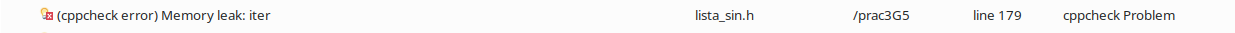
\includegraphics[scale=0.38]{img/captura43.png}
				\caption{Detalle del mensaje de error de cppcheck}
				\label{captura43}
			\end{figure}
		
			\begin{figure}[H]
				\centering
				
\includegraphics[scale=0.38]{img/captura46.png}
				\caption{Detalle del mensaje de error de cppcheck}
				\label{captura46}
			\end{figure}
			
			\paragraph{}El error se origina cuando, en la línea 179, hacemos que la variable \textit{iter} (que es un puntero) apunte al atributo de la clase \textit{primero} sin liberar la memoria de la estructura con la que inicializamos anteriormente. Esto hace que la memoria que ocupa dicha estructura no se libere y que, por lo tanto, se produzca una pérdida de memoria. 
			
			\paragraph{}En el caso de la función \textit{elimina\_dao}, la explicación del origen del error es exactamente la misma pero aplicada a la variable \textit{viejo}.
		
		\subsubsection{Corrección realizada para solventar el error}
		
			\paragraph{}La manera de resolver esta incidencia es de lo más trivial. Tan solo deberemos realizar la declaración de la variable y, acto seguido, asignarle la dirección de memoria del atributo de la clase \textit{primero}. A continuación, dejamos una captura de pantalla del estado de las funciones tras la resolución de los errores:
			
			\begin{figure}[H]
				\centering
				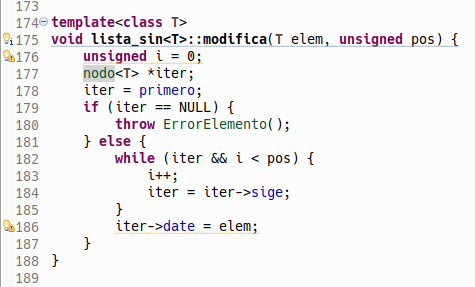
\includegraphics[scale=0.7]{img/captura44.png}
				\caption{Captura de pantalla de la función modifica tras la resolución del error}
				\label{captura44}
			\end{figure}
		
			\begin{figure}[H]
				\centering
				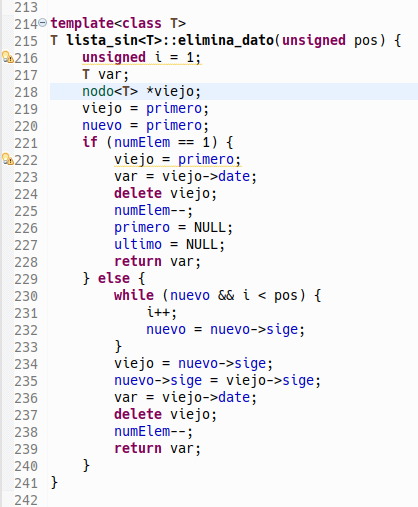
\includegraphics[scale=0.7]{img/captura47.png}
				\caption{Captura de pantalla de la función elimina\_dato}
				\label{captura47}
			\end{figure}
		
			\paragraph{nota:}Cabe destacar que también se podría haber resuelto este error realizando un $"delete$ $iter/viejo"$ antes de asignarle la dirección de memoria del atributo \textit{primero} pero en este caso hemos descartado esta opción ya que la estructura con la que se inicializa no se utiliza para nada y supondría la realización de operaciones adicionales innecesarias.
	
	\subsection{Error nº2: Mismatching allocation and deallocation}

		\subsubsection{Origen/explicación del error detectado}
		
			\paragraph{}A continuación presentamos una captura de pantalla de la función \textit{limpia} de la clase plantilla \textit{lista\_sin}.
		
			\begin{figure}[H]
				\centering
				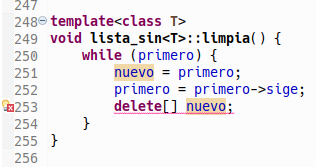
\includegraphics[scale=0.7]{img/captura48.png}
				\caption{Captura de pantalla de la función limpia}
				\label{captura48}
			\end{figure}
	
			\paragraph{}En esta función, en la línea 253, cppcheck nos indica que hay un error. Dicho error es originado dado que hacemos un $"delete[]"$, es decir, una liberación de memoria para un vector/array de punteros. En el caso de la variable \textit{nuevo}, podemos comprobar que se trata de un atributo de la clase \textit{lista\_sin} y que se trata de un puntero a una estructura llamada \textit{nodo}. Justo esto anterior es lo que genera el error, es decir, estamos intentando liberar la memoria asignada de un vector/array cuando la variable \textbf{no es ninguno de estos}.
		
			\begin{figure}[H]
				\centering
				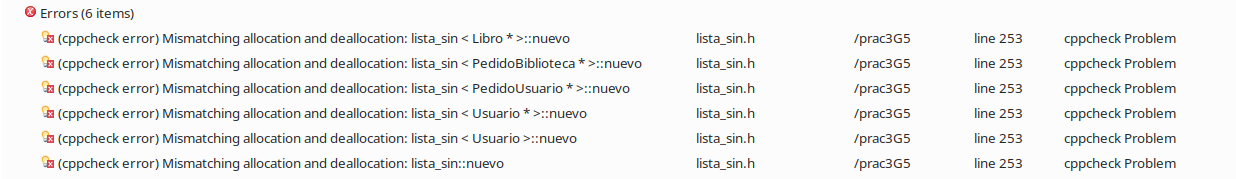
\includegraphics[scale=0.38]{img/captura49.png}
				\caption{Detalle del mensaje de error de cppcheck}
				\label{captura49}
			\end{figure}

		\subsubsection{Corrección realizada para solventar el error}
		
			\paragraph{}Para corregir este error lo único que deberemos realizar es sustituir la sentencia $"delete[]$ $nuevo"$ por la sentencia $"delete$ $nuevo"$. Una vez realizado esto el error habrá desaparecido, como se puede comprobar en la siguiente captura de pantalla:
		
			\begin{figure}[H]
				\centering
				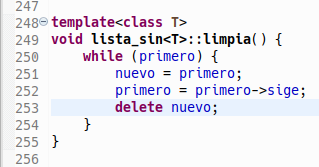
\includegraphics[scale=0.7]{img/captura50.png}
				\caption{Captura de pantalla de la función limpia tras la resolución del error}
				\label{captura50}
			\end{figure}
		
	\subsection{Error nº3: Class has a constructor with 1 argument that is not explicit}
	
		\subsubsection{Origen/explicación del error detectado}
	
			\paragraph{}En la siguiente captura de pantalla se observa el constructor parametrizado de la clase \textit{PedidoBiblioteca}.
			
			\begin{figure}[H]
				\centering
				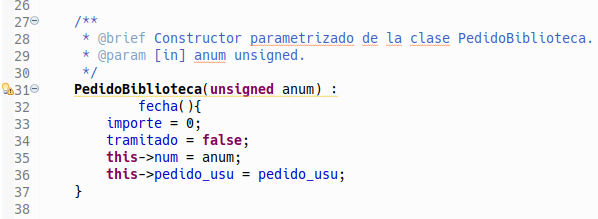
\includegraphics[scale=0.7]{img/captura51.png}
				\caption{Captura de pantalla del constructor parametrizado de la clase PedidoBiblioteca}
				\label{captura51}
			\end{figure}
		
			\paragraph{}Como se puede observar en la captura de pantalla, en este constructor se hace uso de una lista de inicializadores de miembro, la cual inicializa el valor de los atributos miembro antes de la ejecución del cuerpo del constructor.
			
			\paragraph{}En la lista observamos que se encuentra el atributo miembro \textit{fecha} inicializado con su constructor por defecto. Esto es debido a que entre paréntesis no hemos escrito ningún nombre de variable, ya que no se le pasa ningún parámetro del tipo fecha al constructor.
			
			\paragraph{}No obstante, el parámetro \textit{anum} no se usa en la lista, sino que se usa posteriormente en el cuerpo del constructor. Aquí es donde se haya el origen del error.
			
			\paragraph{}Como bien hemos estudiado en los primeros cursos de la carrera, cuando usamos la lista de inicializadores de miembro, es común asignar un valor por defecto a todos los parámetros del constructor. De este modo, si no se le pasara algún parámetro a este constructor, incializaría el atributo miembro con el valor por defecto que tenga declarado el parámetro en cuestión.
			
			\paragraph{}El parámetro \textit{anum} no tiene ningún valor por defecto y es por este motivo que la herramienta cppcheck nos genera el error. 
			
			\begin{figure}[H]
				\centering
				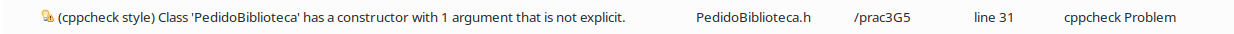
\includegraphics[scale=0.38]{img/captura52.png}
				\caption{Detalle del mensaje de error de cppcheck}
				\label{captura52}
			\end{figure}
	
	\subsubsection{Corrección realizada para solventar el error}
	
			\paragraph{}La forma de corregir el error generado es muy sencilla. Nos limitaremos a asignarle un valor por defecto al parámetro \textit{anum}, en este caso el mismo valor que se le asigna al atributo miembro \textit{num} en el constructor por defecto. De este modo, podremos comprobar que el error habrá desaparecido.
			
			\begin{figure}[H]
				\centering
				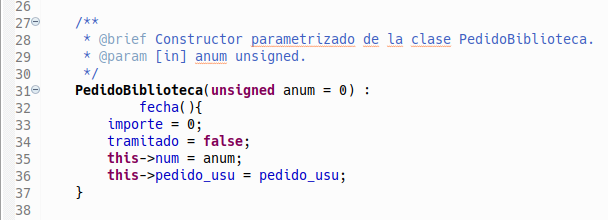
\includegraphics[scale=0.7]{img/captura53.png}
				\caption{Captura de pantalla del constructor parametrizado de la clase PedidoBiblioteca tras la corrección del error}
				\label{captura53}
			\end{figure}
		
			\paragraph{Nota:} Una segunda forma de corregir el error habría sido declarar el constructor como explícito, es decir, añadir \textit{explicit} a la declaración del constructor. Hemos descartado esta opción ya que en algunos casos esto podría ocasionar un comportamiento indeseado en la ejecución del programa en ciertas situaciones.

	\subsection{Error nº4: Parameter can be declared with const}
	
		\subsubsection{Origen/explicación del error detectado}
		
		\paragraph{}Este error tiene su origen en el constructor por copia de la clase \textit{PedidoBiblioteca}. A continuación, se presenta una captura de pantalla de dicho constructor.
		
		\begin{figure}[H]
			\centering
			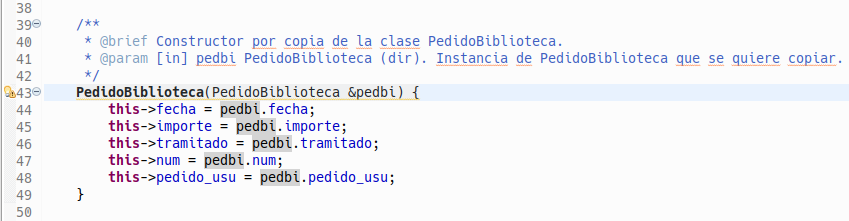
\includegraphics[scale=0.55]{img/captura54.png}
			\caption{Captura de pantalla del constructor por copia de la clase PedidoBiblioteca}
			\label{captura54}
		\end{figure}
	
		\paragraph{}Como se puede observar en la captura, cppcheck nos indica que el error se encuentra en la línea 43 del archivo. Nos recomienda que el parámetro \textit{pedbi} puede ser declarado como constante. Este parámetro es el la instancia del objeto del cuál se hace una copia
		
		\paragraph{}Es bastante común (y recomendable) que en los constructores por copia y en los operadores de asignación se pasen como constante los objetos de los cuales queremos copiar el valor de sus atributos. Esto se realiza para evitar que, bien por descuido o bien por error de programación, se modifiquen los valores de los atributos miembros de estos parámetros.
		
		\paragraph{}Es por este motivo que cppcheck nos avisa de que podemos hacer este parámetro constante.
		
		\paragraph{}Este error también es detectado para el parámetro \textit{pedbi}, en la línea 70 del archivo \textit{PedidoBiblioteca.h}; y para el parámetro \textit{pedido}, en la línea 49 del archivo \textit{PedidoUsuario.h}. A continuación, presentamos capturas de pantalla de las funciones en las que aparecen estos errores.
		
		\begin{figure}[H]
			\centering
			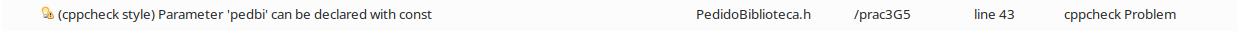
\includegraphics[scale=0.38]{img/captura55.png}
			\caption{Detalle del mensaje de error de cppcheck}
			\label{captura55}
		\end{figure}
	
		\begin{figure}[H]
			\centering
			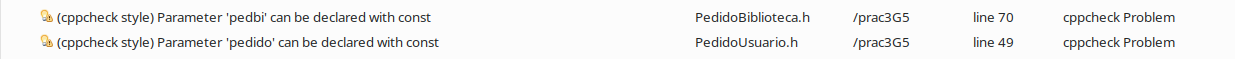
\includegraphics[scale=0.38]{img/captura61.png}
			\caption{Detalle del mensaje de error de cppcheck}
			\label{captura61}
		\end{figure}
	
		\begin{figure}[H]
			\centering
			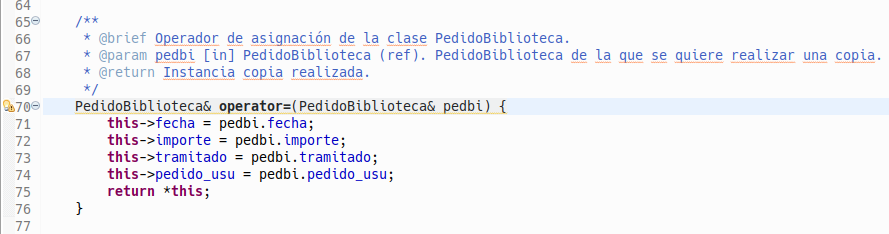
\includegraphics[scale=0.5]{img/captura57.png}
			\caption{Captura de pantalla del operador de asignación de la clase PedidoBiblioteca}
			\label{captura57}
		\end{figure}
	
		\begin{figure}[H]
			\centering
			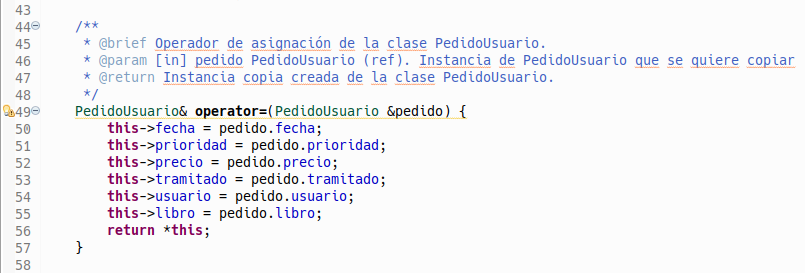
\includegraphics[scale=0.55]{img/captura58.png}
			\caption{Captura de pantalla del operador de asignación de la clase PedidoUsuario}
			\label{captura58}
		\end{figure}
	
		\subsubsection{Corrección realizada para solventar el error}
		
		\paragraph{}Para corregir este error tan solo deberemos hacer constante el parámetro \textit{pedbi}. Una vez hecho esto habrá desaparecido el aviso de cppcheck.
		
		\begin{figure}[H]
			\centering
			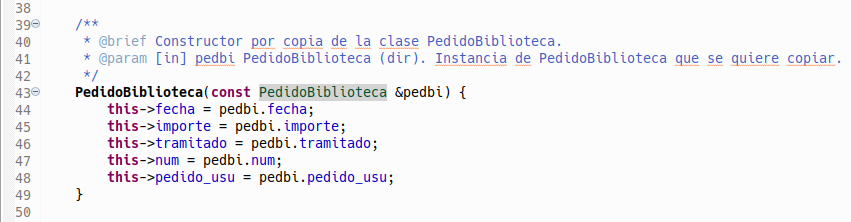
\includegraphics[scale=0.55]{img/captura56.png}
			\caption{Captura de pantalla del constructor por copia de la clase PedidoBiblioteca tras la corrección del error}
			\label{captura56}
		\end{figure}
	
		\begin{figure}[H]
			\centering
			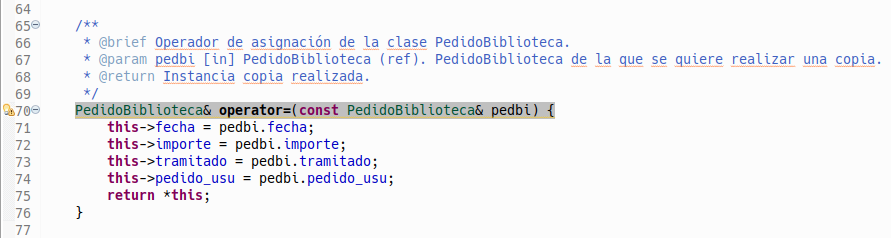
\includegraphics[scale=0.5]{img/captura59.png}
			\caption{Captura de pantalla del operador de asignación de la clase PedidoBiblioteca tras la resolución del error}
			\label{captura59}
		\end{figure}
	
		\paragraph{Nota:}El aviso que se muestra en la captura de pantalla se debe a otro origen; el error de este apartado ha sido solucionado.
		
		\begin{figure}[H]
			\centering
			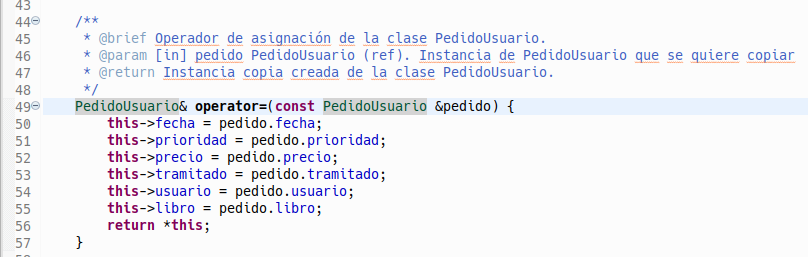
\includegraphics[scale=0.55]{img/captura60.png}
			\caption{Captura de pantalla del operador de asignación de la clase PedidoUsuario tras la resolución del error}
			\label{captura60}
		\end{figure}
		
		\paragraph{Nota:}En el caso de que en nuestro constructor ó función necesitáramos por algún motivo modificar el valor de alguno de los atributos miembro del parámetro y, aún así, nos saltara el aviso de cppcheck deberíamos hacer caso omiso ya que de este modo nos daría un error al compilar el código.
		
	\subsection{Error nº5: The function is never used}
		
		\subsubsection{Origen/explicación del error detectado}
		
			\paragraph{}En este caso, cppcheck nos indica que las siguientes funciones no son utilizadas en nuestro código:
			
			\begin{itemize}
				\item \textit{anadirAnios, anadirDias, anadirHoras, anadirMeses, anadirMin, asignarDia y asignarHora} del archivo \textit{Fecha.cpp}.
				\item \textit{daISBN} del archivo \textit{Libro.cpp}.
				\item \textit{daLBiblioteca} del archivo \textit{Biblioteca.cpp}.
				\item \textit{daLibro} del archivo \textit{PedidoUsuario.cpp}.
				\item \textit{daPedidoUsuario} del archivo \textit{PedidoBiblioteca.cpp}.
				\item \textit{validarClave} del archivo \textit{Usuario.cpp}.
			\end{itemize}
		
			\paragraph{}En el caso de este error explicar el origen de este error resulta de lo más trivial. Las funciones anteriormente enumerada se han definido en sus respectivos archivos y no se llegan a utilizar en el código del programa.
			
			\paragraph{}Por este motivo cppcheck nos alerta de este evento para, en el caso pertinente, eliminar el código fuente de estas funciones y reducir el número de líneas de código de nuestro programa.
		
			\begin{figure}[H]
				\centering
				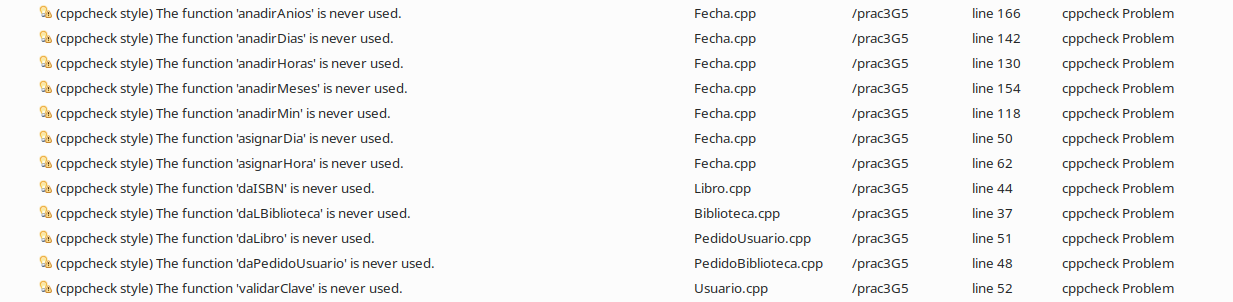
\includegraphics[scale=0.38]{img/captura62.png}
				\caption{Detalle del mensaje de error de cppcheck}
				\label{captura62}
			\end{figure}
		
		\subsubsection{Corrección realizada para solventar el error}
		
			\paragraph{}En nuestro caso particular resolvemos este error indicándole a cppcheck que ignore estos errores. El motivo de tomar tal decisión es debido a que, si bien en el programa no se utilizan estas funciones, en un futuro podrían ser de gran utilidad debido a la naturaleza de las mismas (modificar, obtener y validar atributos de las clases).
			
			\paragraph{}Si bien es cierto que se trata de un programa de granja realizado en el contexto de una práctica de asignatura de la carrera, hemos aplicado un punto de vista simulando que la aplicación se encuentra en producción, que está mantenida y que tendrá futuras actualizaciones de funcionalidades.
			
			\paragraph{}Una vez ignorados los errores no volverán a ser listados por cppcheck.
			
			\paragraph{Nota:}No hemos incluido capturas de pantalla ya que las funciones no presentan ningún error como tal y solo se mostrarían los avisos de cppcheck, haciendo aumentar considerablemente la extensión del presente documento.
			
	\subsection{Error nº6: The scope of the variable can be reduced}
	
		\subsubsection{Origen/explicación del error detectado}
		
			\paragraph{}Para este error, cppcheck nos lista 11 incidencias, las cuales mostramos a continuación a modo de captura de pantalla.
			
			\begin{figure}[H]
				\centering
				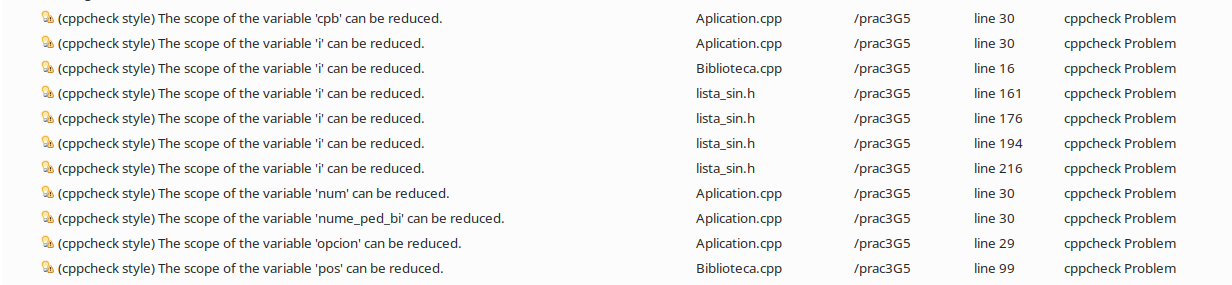
\includegraphics[scale=0.38]{img/captura63.png}
				\caption{Detalle del mensaje de error de cppcheck}
				\label{captura63}
			\end{figure}
		
			\paragraph{}Todos los errores que se generan tienen su origen en la declaración al inicio de la función de las variables para, más adelante, ser inicializadas cuando vayan a utilizarse.
			
			\paragraph{}Es recomendable que se declaren e inicialicen las variables locales de una función justo en el fragmento de código en el que vayan a ser utilizados. Por ejemplo, en vez de definir la variable iteradora 'i' de un bucle \textit{for} al inicio de la función y asignarle el valor inicial en el bucle, se debe inicializar y asignar el valor en el mismo bucle.
			
			\paragraph{}En todas las capturas de pantalla siguientes se puede observar cómo cppcheck nos indica que cometemos este error en todas las variables resaltadas.
			
			\begin{figure}[H]
				\centering
				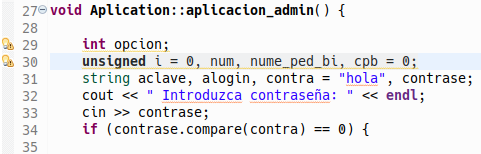
\includegraphics[scale=0.7]{img/captura64.png}
				\caption{Captura de pantalla del error cppcheck en el código fuente}
				\label{captura64}
			\end{figure}
		
			\begin{figure}[H]
				\centering
				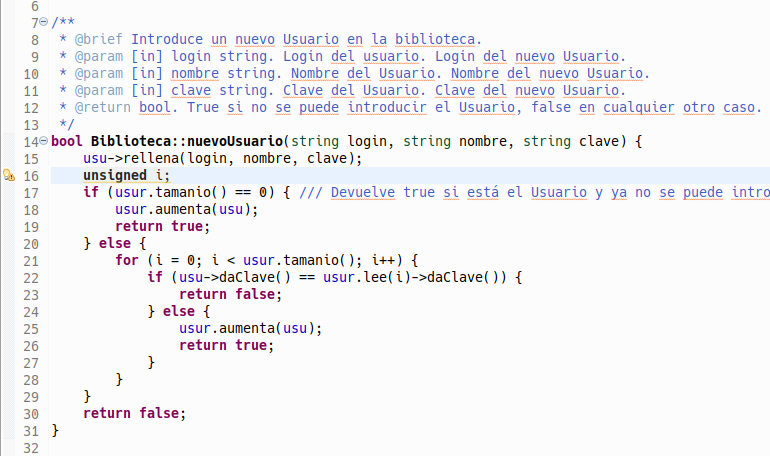
\includegraphics[scale=0.55]{img/captura65.png}
				\caption{Captura de pantalla del error cppcheck en el código fuente}
				\label{captura65}
			\end{figure}
		
			\begin{figure}[H]
				\centering
				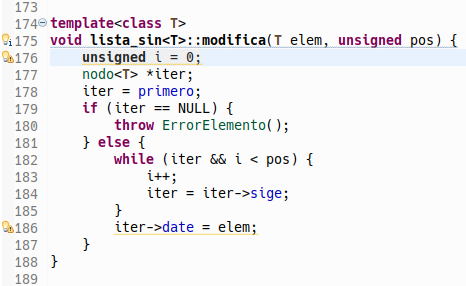
\includegraphics[scale=0.55]{img/captura66.png}
				\caption{Captura de pantalla del error cppcheck en el código fuente}
				\label{captura66}
			\end{figure}
		
			\begin{figure}[H]
				\centering
				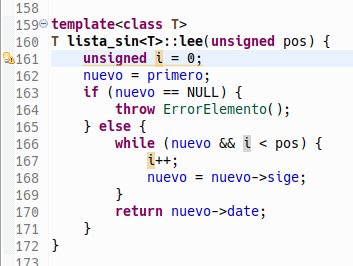
\includegraphics[scale=0.55]{img/captura74.png}
				\caption{Captura de pantalla del error cppcheck en el código fuente}
				\label{captura74}
			\end{figure}
		
			\begin{figure}[H]
				\centering
				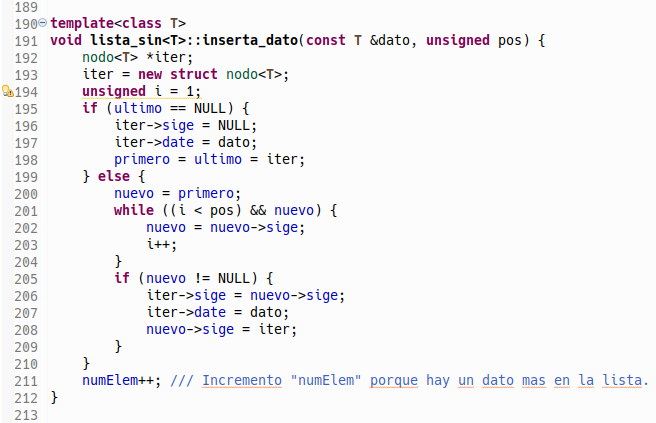
\includegraphics[scale=0.55]{img/captura67.png}
				\caption{Captura de pantalla del error cppcheck en el código fuente}
				\label{captura67}
			\end{figure}
		
			\begin{figure}[H]
				\centering
				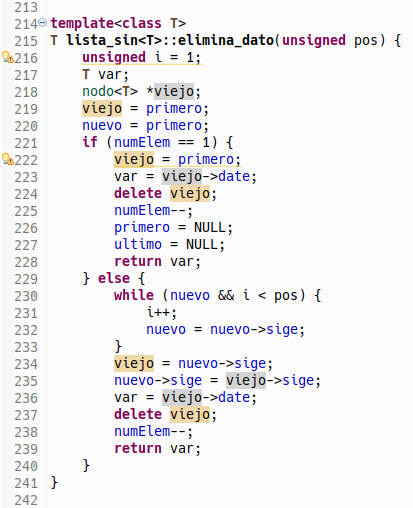
\includegraphics[scale=0.55]{img/captura68.png}
				\caption{Captura de pantalla del error cppcheck en el código fuente}
				\label{captura68}
			\end{figure}
		
			\begin{figure}[H]
				\centering
				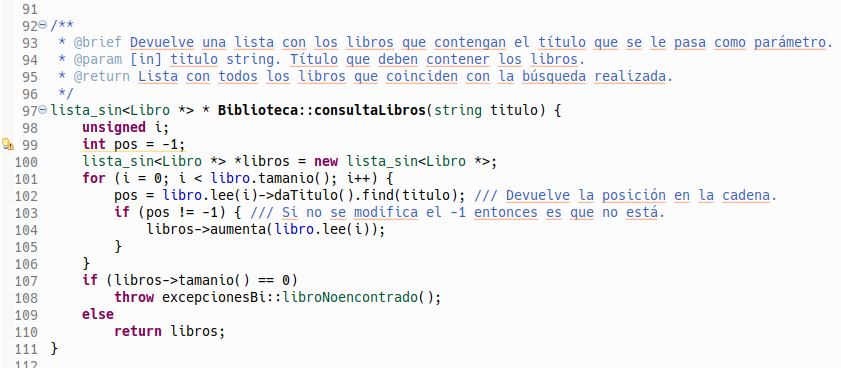
\includegraphics[scale=0.55]{img/captura69.png}
				\caption{Captura de pantalla del error cppcheck en el código fuente}
				\label{captura69}
			\end{figure}
		
		\subsubsection{Corrección realizada para solventar el error}
		
			\paragraph{}Para el error existente en la línea 29 de la figura \ref*{captura64} la solución consistirá en realizar la declaración  dentro del bloque \textit{if} de la función.
			
			\begin{figure}[H]
				\centering
				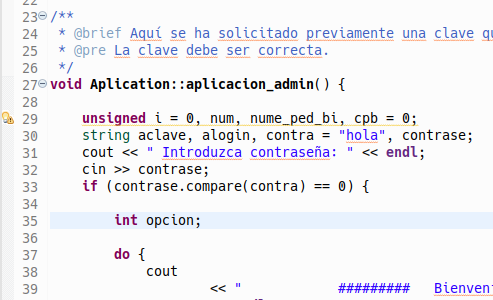
\includegraphics[scale=0.7]{img/captura70.png}
				\caption{Captura de pantalla del error cppcheck  resuelto en el código fuente}
				\label{captura70}
			\end{figure}
	
			\paragraph{}Para el error que hace referencia a la variable \textit{cpb} existente en la línea 30 de la figura \ref*{captura64} la solución consistirá en realizar la declaración e inicialización dentro del bloque \textit{switch - case} de la función.
			
			\begin{figure}[H]
				\centering
				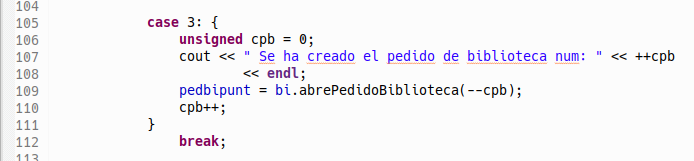
\includegraphics[scale=0.6]{img/captura71.png}
				\caption{Captura de pantalla del error cppcheck  resuelto en el código fuente}
				\label{captura71}
			\end{figure}
		
			\paragraph{}Para el error que hace referencia a la variable \textit{i} existente en la línea 30 de la figura \ref*{captura64} la solución consistirá en realizar la declaración e inicialización dentro del bloque \textit{switch - case} de la función.
			
			\begin{figure}[H]
				\centering
				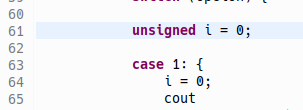
\includegraphics[scale=0.7]{img/captura72.png}
				\caption{Captura de pantalla del error cppcheck  resuelto en el código fuente}
				\label{captura72}
			\end{figure}
		
			\paragraph{}Para el error que hace referencia a la variable \textit{i} existente en la línea 16 de la figura \ref*{captura65} la solución consistirá en realizar la declaración e inicialización dentro del bucle \textit{for} de la función.
			
			\begin{figure}[H]
				\centering
				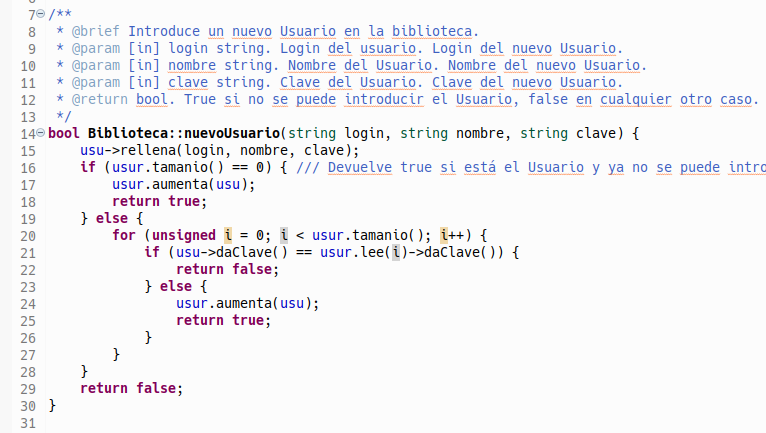
\includegraphics[scale=0.6]{img/captura73.png}
				\caption{Captura de pantalla del error cppcheck  resuelto en el código fuente}
				\label{captura73}
			\end{figure}
		
			\paragraph{}Para el error que hace referencia a la variable \textit{i} existente en la línea 161 de la figura \ref*{captura74} la solución consistirá en realizar la declaración e inicialización dentro del bloque \textit{else} de la función.
			
			\begin{figure}[H]
				\centering
				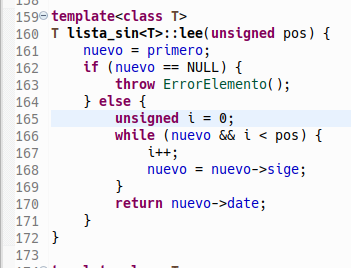
\includegraphics[scale=0.7]{img/captura75.png}
				\caption{Captura de pantalla del error cppcheck  resuelto en el código fuente}
				\label{captura75}
			\end{figure}
		
			\paragraph{}Para el error que hace referencia a la variable \textit{i} existente en la línea 176 de la figura \ref*{captura66} la solución consistirá en realizar la declaración e inicialización dentro del bloque \textit{else} de la función.
			
			\begin{figure}[H]
				\centering
				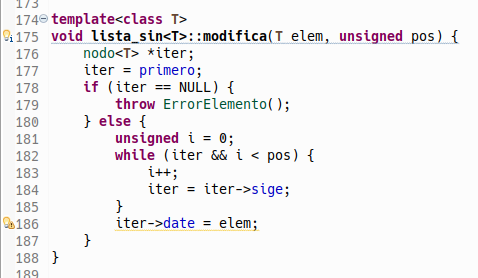
\includegraphics[scale=0.7]{img/captura76.png}
				\caption{Captura de pantalla del error cppcheck  resuelto en el código fuente}
				\label{captura76}
			\end{figure}
		
			\paragraph{}Para el error que hace referencia a la variable \textit{i} existente en la línea 194 de la figura \ref*{captura67} la solución consistirá en realizar la declaración e inicialización dentro del bloque \textit{else} de la función.
			
			\begin{figure}[H]
				\centering
				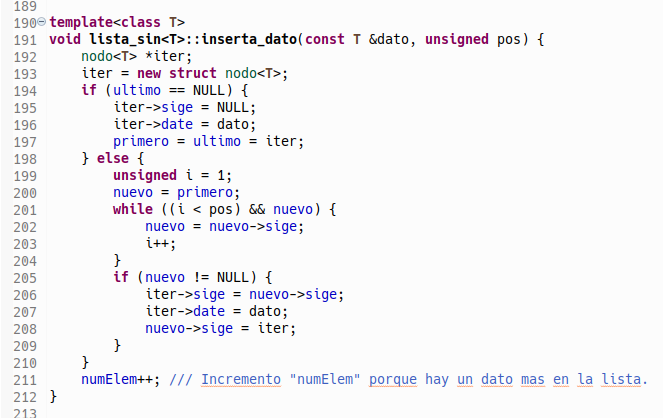
\includegraphics[scale=0.7]{img/captura77.png}
				\caption{Captura de pantalla del error cppcheck  resuelto en el código fuente}
				\label{captura77}
			\end{figure}
		
			\paragraph{}Para el error que hace referencia a la variable \textit{i} existente en la línea 216 de la figura \ref*{captura68} la solución consistirá en realizar la declaración e inicialización dentro del bloque \textit{else} de la función.
			
			\begin{figure}[H]
				\centering
				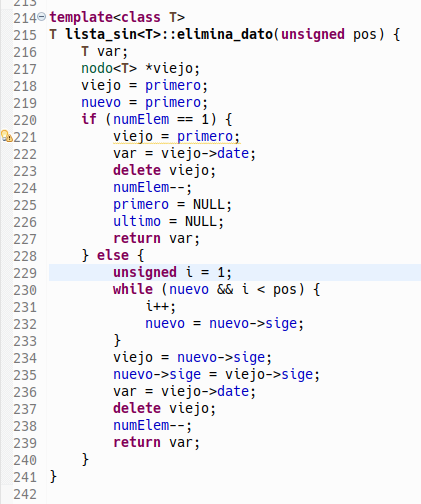
\includegraphics[scale=0.7]{img/captura78.png}
				\caption{Captura de pantalla del error cppcheck  resuelto en el código fuente}
				\label{captura78}
			\end{figure}
		
			\paragraph{}Para el error que hace referencia a la variable \textit{num} existente en la línea 30 de la figura \ref*{captura64} la solución consistirá en realizar la declaración e inicialización dentro del bloque \textit{switch - case} de la función.
			
			\begin{figure}[H]
				\centering
				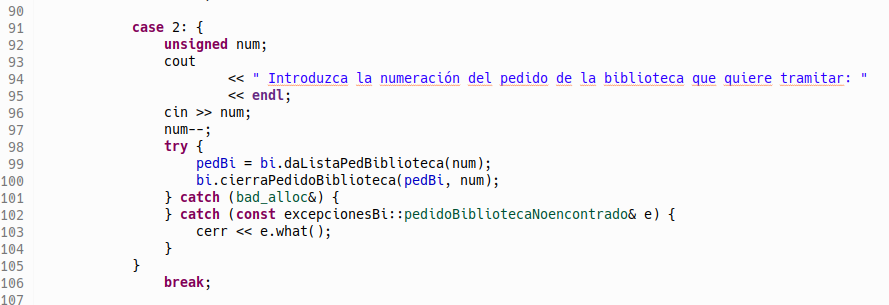
\includegraphics[scale=0.5]{img/captura79.png}
				\caption{Captura de pantalla del error cppcheck  resuelto en el código fuente}
				\label{captura79}
			\end{figure}
		
			\paragraph{}Para el error que hace referencia a la variable \textit{nume\_ped\_bi} existente en la línea 30 de la figura \ref*{captura64} la solución consistirá en realizar la declaración e inicialización dentro del bloque \textit{switch - case} de la función.
			
			\begin{figure}[H]
				\centering
				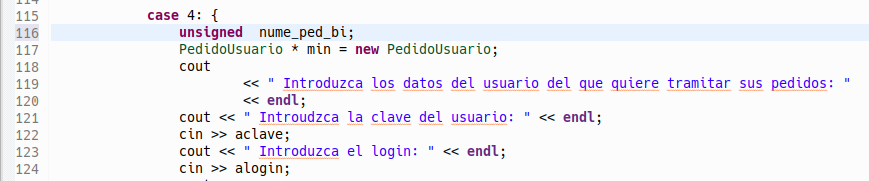
\includegraphics[scale=0.5]{img/captura80.png}
				\caption{Captura de pantalla del error cppcheck  resuelto en el código fuente}
				\label{captura80}
			\end{figure}
		
			\paragraph{}Para el error que hace referencia a la variable \textit{pos} existente en la línea 98 de la figura \ref*{captura69} la solución consistirá en realizar la declaración e inicialización dentro del bucle \textit{for} de la función.
			
			\begin{figure}[H]
				\centering
				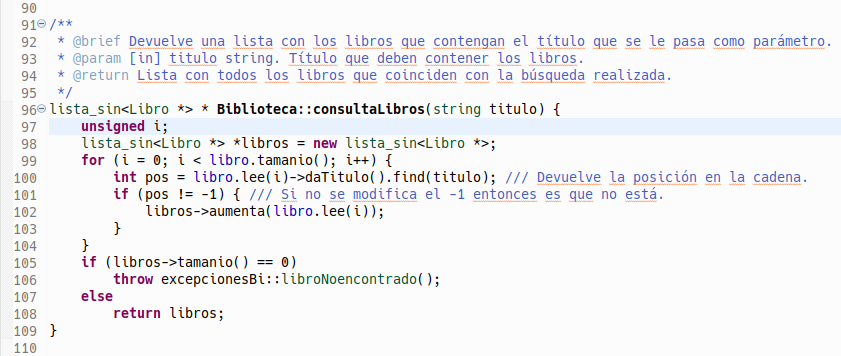
\includegraphics[scale=0.55]{img/captura81.png}
				\caption{Captura de pantalla del error cppcheck  resuelto en el código fuente}
				\label{captura81}
			\end{figure}
		
	\subsection{Error nº7: Unused varriable}
	
		\subsubsection{Origen/explicación del error detectado}
		
		\paragraph{}Cppcheck nos indica en este caso que el error se origina en la línea 232 del archivo \textit{Application.cpp}, más concretamente en la variable \textit{basura}.
		
		\begin{figure}[H]
			\centering
			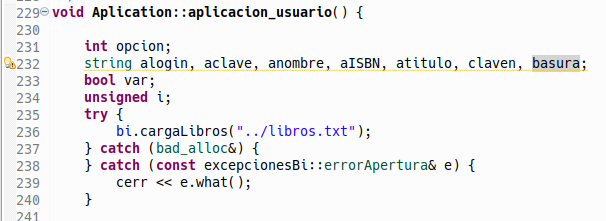
\includegraphics[scale=0.55]{img/captura82.png}
			\caption{Captura de pantalla del error cppcheck en el código fuente}
			\label{captura82}
		\end{figure}
	
		\paragraph{}El error se origina debido a que declaramos esta variable pero no llegamos a utilizarla en toda la función, generando en consecuencia un desperdicio de la memoria local de la función. Por este motivo, cppcheck nos alerta al respecto.
	
		\begin{figure}[H]
			\centering
			
\includegraphics[scale=0.38]{img/captura83.png}
			\caption{Detalle del mensaje de error de cppcheck}
			\label{captura83}
		\end{figure}
		
		\subsubsection{Corrección realizada para solventar el error}
		
		\paragraph{}La resolución de este error consiste en la eliminación de dicha variable de nuestro código. Una vez realizado esto, el error habrá sido eliminado.
		
		\begin{figure}[H]
			\centering
			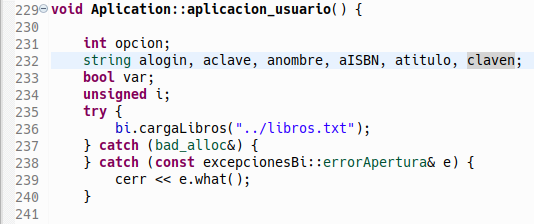
\includegraphics[scale=0.55]{img/captura84.png}
			\caption{Captura de pantalla del error cppcheck resuelto en el código fuente}
			\label{captura84}
		\end{figure}
	
	\subsection{Error nº8: Variable is reassigned a value before the old one has been used}
	
	\subsubsection{Origen/explicación del error detectado}
	
		\paragraph{}Este error tiene su origen en la línea 221 del archivo \textit{lista\_sin.h}.
	
		\begin{figure}[H]
			\centering
			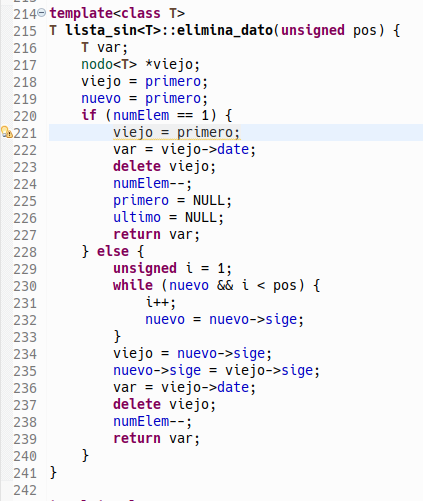
\includegraphics[scale=0.55]{img/captura86.png}
			\caption{Captura de pantalla del error cppcheck en el código fuente}
			\label{captura86}
		\end{figure}
	
		\paragraph{}Este error se origina cuando, tras declarar la variable \textit{viejo} en la línea 217, se le asigna la dirección de memoria que hay guardada en la variable \textit{primero} (línea 218).
		
		\paragraph{}Una vez que hemos hecho esto, en la línea 221 volvemos a asignarle el valor de \textit{primero}. En nuestro código no habría problema, pero si en la primera asignación le hubiéramos pasado otro valor no habríamos llegado a realizar ninguna operación con este primer valor. Es decir, hemos guardado una información que no hemos utilizado para nada. En consecuencia, habremos realizado una operación innecesaria (primera asignación). Este es el porqué de que cppcheck nos lance una advertencia al respecto.
		\begin{figure}[H]
			\centering
			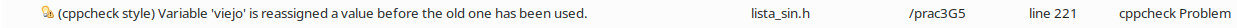
\includegraphics[scale=0.38]{img/captura85.png}
			\caption{Detalle del mensaje de error de cppcheck}
			\label{captura85}
		\end{figure}
	
	\subsubsection{Corrección realizada para solventar el error}
	
		\paragraph{}La solución a este error pasa por eliminar la segunda asignación del código fuente (línea 221), ya que la primera asignación es válida al entrar en la ejecución del bloque \textit{if}. De este modo, el error habrá sido solventado.
		
		\begin{figure}[H]
			\centering
			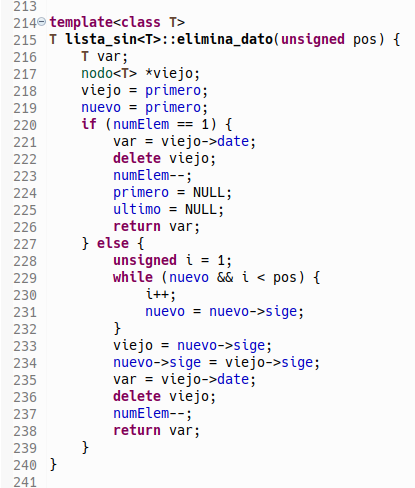
\includegraphics[scale=0.55]{img/captura87.png}
			\caption{Captura de pantalla del error cppcheck resuelto en el código fuente}
			\label{captura87}
		\end{figure}
	
	\subsection{Error nº9: Either the condition is redundant or there is possible null pointer dereference}
	
		\subsubsection{Origen/explicación del error detectado}
		
			\paragraph{}Este error se encuentra en la línea 186 del archivo \textit{lista\_sin.h}, en la siguiente captura de pantalla se muestra la función en la que se encuentra dicho error.
		
			\begin{figure}[H]
				\centering
				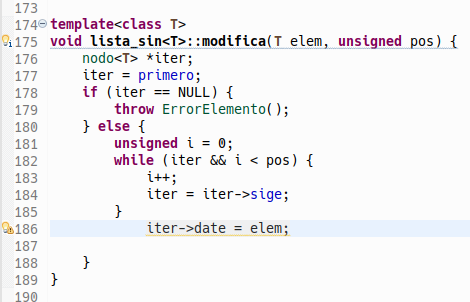
\includegraphics[scale=0.55]{img/captura89.png}
				\caption{Captura de pantalla del error cppcheck en el código fuente}
				\label{captura89}
			\end{figure}
		
			\paragraph{}Este error es causado porque no comprobamos que el puntero \textit{iter} no esté apuntando a NULL. En otra situación, estando \textit{iter} inicializado correctamente, no hubiera sido necesario realizar esta comprobación pero, como se puede observar en la captura de pantalla, dentro del bucle \textit{while} se va actualizando la dirección a la que apunta con el valor de \textit{sige}. 
			
			\paragraph{}Al final de la ejecución del bucle \textit{while} es posible que \textit{iter} esté apuntando a NULL, de hecho una de las condiciones de parada del bucle es que esté apuntando a NULL. Por este motivo cppcheck nos alerta de este hecho.
		
			\begin{figure}[H]
				\centering
				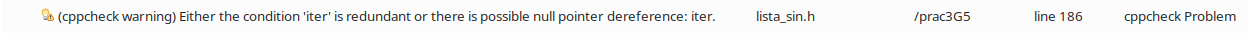
\includegraphics[scale=0.38]{img/captura88.png}
				\caption{Detalle del mensaje de error de cppcheck}
				\label{captura88}
			\end{figure}
		
		\subsubsection{Corrección realizada para solventar el error}
		
			\paragraph{}La manera de subsanar este error es realizar la comprobación de que no esté apuntando a NULL justo antes de acceder al objeto apuntado. En la captura de pantalla que se encuentra a continuación se puede observar con detalle la solución aplicada.
			
			\begin{figure}[H]
				\centering
				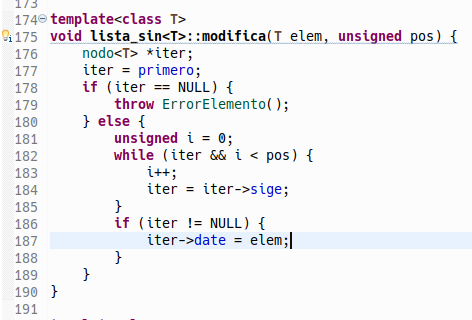
\includegraphics[scale=0.55]{img/captura90.png}
				\caption{Captura de pantalla del error cppcheck subsanado en el código fuente}
				\label{captura90}
			\end{figure}
		
	\subsection{Error nº10: Possible leak in public function. The pointer is not deallocated before is allocated}
	
		\subsubsection{Origen/explicación del error detectado}
		
			\paragraph{}En la siguiente captura de pantalla se muestra la función que contiene el error de cppcheck.
		
			\begin{figure}[H]
				\centering
				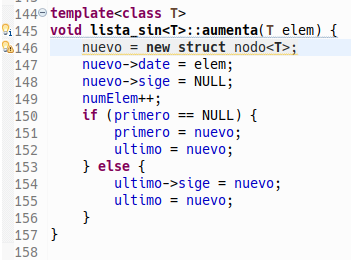
\includegraphics[scale=0.55]{img/captura91.png}
				\caption{Captura de pantalla del error cppcheck en el código fuente}
				\label{captura91}
			\end{figure}
		
			\paragraph{}Se puede observar que en la línea 146 se le asigna la dirección de memoria de un nuevo \textit{nodo} al puntero \textit{nuevo}. \textit{nuevo} es un atributo miembro de la clase y es posible que ya estuviera apuntando a otra dirección de memoria y, por lo tanto, es posible que se esté produciendo una fuga de memoria. Es por esto que cppcheck nos lanza la advertencia.
		
			\begin{figure}[H]
				\centering
				\includegraphics[scale=0.38]{img/captura92.png}
				\caption{Detalle del mensaje de error de cppcheck}
				\label{captura92}
			\end{figure}
	
		\subsubsection{Corrección realizada para solventar el error}
		
			\paragraph{}En la captura de pantalla siguiente se puede observar la solución aplicada al código fuente para solventar el error. Esta solución consiste en liberar la memoria de \textit{nuevo}, previa comprobación de que no esté apuntando a NULL para evitar posibles errores.
		
			\begin{figure}[H]
				\centering
				\includegraphics[scale=0.55]{img/captura93.png}
				\caption{Captura de pantalla del error cppcheck subsanado en el código fuente}
				\label{captura9}
			\end{figure}
		
	\subsection{Warning Nº 1}
	
		\subsubsection{Origen/explicación del warning detectado:}
		
			\begin{figure}[H]
				\centering
				\includegraphics[scale=0.55]{img/esteban1.png}
				\label{esteban1}
			\end{figure}
		
			\paragraph{}Se observa el warning en la línea 16 que nos informa que 
			
		\subsubsection{Corrección realizada para solventar el warning:}
		
			\paragraph{}Captura de pantalla
			
	\subsection{Warning Nº 5}
	
		\subsubsection{Origen/explicación del warning detectado:}
		
			\begin{figure}[H]
				\centering
				\includegraphics[scale=0.55]{img/esteban2.png}
				\label{esteban2}
			\end{figure}
		
			\paragraph{}Se observa el warning en la línea seleccionada que nos informa que la variable miembro anio no tiene asignado valor en el operador de igualdad.
			
		\subsubsection{Corrección realizada para solventar el warning:}
		
			\begin{figure}[H]
				\centering
				\includegraphics[scale=0.55]{img/esteban3.png}
				\label{esteban3}
			\end{figure}
		
			\paragraph{}Se coloca dentro del operador de igualdad para que la variable miembro anio pueda tener un valor asignado.
			
	\subsection{Warning Nº 6}
	
		\subsubsection{Origen/explicación del warning detectado:}
		
			\begin{figure}[H]
				\centering
				\includegraphics[scale=0.55]{img/esteban4.png}
				\label{esteban4}
			\end{figure}
		
			\paragraph{}Se observa el warning en la línea seleccionada que nos informa que la variable miembro precioActual no tiene asignado valor en el operador de igualdad.
			
		\subsubsection{Corrección realizada para solventar el warning:}
		
			\begin{figure}[H]
				\centering
				\includegraphics[scale=0.55]{img/esteban5.png}
				\label{esteban5}
			\end{figure}
		
			\paragraph{}Se coloca dentro del operador de igualdad para que precioActual pueda tener un valor asignado.
			
	\subsection{Warning Nº 7}
		
		\subsubsection{Origen/explicación del warning detectado:}
		
			\begin{figure}[H]
				\centering
				\includegraphics[scale=0.55]{img/esteban6.png}
				\label{esteban6}
			\end{figure}
		
			\paragraph{}En este warning en la línea seleccionada que nos informa que la variable miembro numElem no tiene asignado valor en el operador de igualdad.
			
		\subsubsection{Corrección realizada para solventar el warning:}
		
			\begin{figure}[H]
				\centering
				\includegraphics[scale=0.55]{img/esteban7.png}
				\label{esteban7}
			\end{figure}
		
			\paragraph{}Se coloca dentro del operador de igualdad para que numElem pueda tener un valor asignado.
			
	\subsection{Warning Nº 13}
	
		\subsubsection{Origen/explicación del warning detectado:}
		
			\paragraph{}En este warning en la línea seleccionada que nos informa que la variable miembro num de la clase PedidoBiblioteca no tiene asignado valor en el operador de igualdad.
			
			\begin{figure}[H]
				\centering
				\includegraphics[scale=0.55]{img/esteban8.png}
				\label{esteban8}
			\end{figure}
		
		\subsubsection{Corrección realizada para solventar el warning:}
		
			\begin{figure}[H]
				\centering
				\includegraphics[scale=0.55]{img/esteban9.png}
				\label{esteban9}
			\end{figure}
		
			\paragraph{}Se coloca dentro del operador de igualdad para que num pueda tener un valor asignado.
			
	\subsection{INFO N.º 1}
	
		\subsubsection{Origen/explicación del info detectado:}
		
			\paragraph{}En este info se nos informa que Cppcheck no puede encontrar todos los archivos Include.
			
		\subsubsection{Corrección realizada para solventar el info:}
		
	\subsection{INFO N.º 2}
	
		\subsubsection{Origen/explicación del info detectado:}
		
			\begin{figure}[H]
				\centering
				\includegraphics[scale=0.55]{img/esteban10.png}
				\label{esteban10}
			\end{figure}
		
			\paragraph{}En este info se nos informa que el parámetro de la función aTitulo debería ser pasado por referencia constante, al igual que aAutores, aEditorial y aISBN.
			
		\subsubsection{ Corrección realizada para solventar el info:}
		
			\begin{figure}[H]
				\centering
				\includegraphics[scale=0.55]{img/esteban11.png}
				\label{esteban11}
			\end{figure}
		
			\paragraph{}Le hemos añadido la palabra reservada const antes del tipo de las variables.
			
			\paragraph{NOTA}Haciendo esto mismo, hemos logrado eliminar 4 Infos.
			
	\subsection{INFO N.º 6}
	
		\subsubsection{Origen/explicación del info detectado:}
		
			\begin{figure}[H]
				\centering
				\includegraphics[scale=0.55]{img/esteban12.png}
				\label{esteban12}
			\end{figure}
		
			\paragraph{}En este info se nos informa que el parámetro de la función anombre, al igual que alogin y aclave, deberían ser pasados por referencia constante, al igual la info anterior.
			
		\subsubsection{Corrección realizada para solventar el info:}
		
			\begin{figure}[H]
				\centering
				\includegraphics[scale=0.55]{img/esteban13.png}
				\label{esteban13}
			\end{figure}
		
			\paragraph{}Le hemos añadido la palabra reservada const antes del tipo de las variables.
			
			\paragraph{NOTA}Haciendo esto mismo, hemos logrado eliminar otras 2 Infos.
	\subsection{INFO N.º 9}
	
		\subsubsection{Origen/explicación del info detectado:}
		
			\begin{figure}[H]
				\centering
				\includegraphics[scale=0.55]{img/esteban14.png}
				\label{esteban14}
			\end{figure}	
		
			\paragraph{}En este info se nos informa que el parámetro de la función aFecha debería ser pasado por referencia constante, al igual las infos anteriores.
			
		\subsubsection{Corrección realizada para solventar el info:}
		
			\begin{figure}[H]
				\centering
				\includegraphics[scale=0.55]{img/esteban15.png}
				\label{esteban15}
			\end{figure}
		
			\paragraph{}Le hemos añadido la palabra reservada const antes del tipo de la variable.
			
	\subsection{INFO N.º 10}
	
		\subsubsection{Origen/explicación del info detectado:}
		
			\begin{figure}[H]
				\centering
				\includegraphics[scale=0.55]{img/esteban16.png}
				\label{esteban16}
			\end{figure}
		
			\paragraph{}En este info se nos informa que el parámetro de la función login y clave deberían ser pasado s por referencia constante, al igual las infos anteriores.
			
		\subsubsection{Corrección realizada para solventar el info:}
		
			\begin{figure}[H]
				\centering
				\includegraphics[scale=0.55]{img/esteban17.png}
				\label{esteban17}
			\end{figure}
		
			\paragraph{}Le hemos añadido la palabra reservada const antes del tipo de las variables.
			
			\paragraph{NOTA}Haciendo esto mismo, hemos logrado eliminar otras Info.	
			
	\subsection{INFO N.º 12 y N.º 13}
	
		\subsubsection{Origen/explicación de los infos detectados:}
		
			\begin{figure}[H]
				\centering
				\includegraphics[scale=0.55]{img/esteban18.png}
				\label{esteban18}
			\end{figure}
		
			\paragraph{}En estos info se nos informa que los parámetros claven de ambas funciones, deberían ser pasados por referencia constante, al igual que los infos anteriores.
			
		\subsubsection{Corrección realizada para solventar los infos:}
		
			\begin{figure}[H]
				\centering
				\includegraphics[scale=0.55]{img/esteban19.png}
				\label{esteban19}
			\end{figure}
		
			\paragraph{}Le hemos añadido la palabra reservada const antes del tipo de las variables.
			
	\subsection{ INFO N.º 14}
	
		\subsubsection{Origen/explicación de los infos detectados:}
		
			\begin{figure}[H]
				\centering
				\includegraphics[scale=0.55]{img/esteban20.png}
				\label{esteban20}
			\end{figure}
		
			\paragraph{}En este info se nos informa que el parámetro elem, debería ser pasado por referencia constante, al igual que los infos anteriores.
			
		\subsubsection{Corrección realizada para solventar el info:}
		
			\begin{figure}[H]
				\centering
				\includegraphics[scale=0.55]{img/esteban21.png}
				\label{esteban21}
			\end{figure}
		
			\paragraph{}Le hemos añadido la palabra reservada const antes del tipo de la variable y la referencia.
			
	\subsection{INFO N.º 15}
	
		\subsubsection{Origen/explicación de los infos detectados:}
		
			\begin{figure}[H]
				\centering
				\includegraphics[scale=0.55]{img/esteban22.png}
				\label{esteban22}
			\end{figure}
			
			\paragraph{}En este info se nos informa que el parámetro elem, debería ser pasado por referencia constante, al igual que los infos anteriores.
			
		\subsubsection{Corrección realizada para solventar el info:}
		
			\begin{figure}[H]
				\centering
				\includegraphics[scale=0.55]{img/esteban23.png}
				\label{esteban23}
			\end{figure}
		
			\paragraph{}Le hemos añadido la palabra reservada const antes del tipo de la variable y la referencia.
			
	\subsection{INFOS N.º 16 y 17}
	
		\subsubsection{Origen/explicación de los infos detectados:}
		
			\begin{figure}[H]
				\centering
				\includegraphics[scale=0.55]{img/esteban24.png}
				\label{esteban24}
			\end{figure}
		
			\paragraph{}En este info se nos informa que el parámetro aFecha, debería ser pasado por referencia constante, al igual que los infos anteriores, del mismo modo, al solventar este info nos damos cuenta que nos desaparece otro más, el de que la variable fecha es asignada en el cuerpo del constructor y que deberíamos considerar inicializarla en la lista.
			
		\subsubsection{Corrección realizada para solventar los dos infos:}
		
			\begin{figure}[H]
				\centering
				\includegraphics[scale=0.55]{img/esteban25.png}
				\label{esteban25}
			\end{figure}
		
			\paragraph{}Le hemos añadido la palabra reservada const antes del tipo de la variable aFecha junto con su referencia. De este modo, Cppcheck ha considerado que la variable fecha es inicializada en la lista en lugar del cuerpo del constructor y nos ha eliminado dicha info.
			
	\subsection{INFOS N.º 18, 19, 20 y 21}
	
		\subsubsection{Origen/explicación de los infos detectados:}
		
			\begin{figure}[H]
				\centering
				\includegraphics[scale=0.55]{img/esteban26.png}
				\label{esteban26}
			\end{figure}
		
			\paragraph{}En estos cuatro infos se nos informa que las variables título, autores, editorial y ISBN son asignados en el cuerpo del constructor y que deberíamos considerar inicializarlos en la lista.
			
		\subsubsection{Corrección realizada para solventar los cuatro infos:}
		
			\begin{figure}[H]
				\centering
				\includegraphics[scale=0.55]{img/esteban27.png}
				\label{esteban27}
			\end{figure}
		
			\paragraph{}De este modo, Cppcheck ha considerado que las variables anteriores quedan inicializadas en la lista en lugar del cuerpo del constructor y nos ha eliminado dichas infos.
			
	\subsection{INFOS N.º 22, 23 y 24}
	
		\subsubsection{Origen/explicación de los infos detectados:}
		
			\begin{figure}[H]
				\centering
				\includegraphics[scale=0.55]{img/esteban28.png}
				\label{esteban28}
			\end{figure}
		
			\paragraph{}En estos tres infos se nos informa que las variables nombre, clave y login son asignados en el cuerpo del constructor y que deberíamos considerar inicializarlos en la lista.
			
		\subsubsection{Corrección realizada para solventar los tres infos:}
		
			\begin{figure}[H]
				\centering
				\includegraphics[scale=0.55]{img/esteban29.png}
				\label{esteban29}
			\end{figure}
		
			\paragraph{}Al igual que hemos procedido anteriormente, Cppcheck ha considerado que las variables anteriores quedan inicializadas en la lista en lugar del cuerpo del constructor y nos ha eliminado dichas infos.
\newpage